\chapter{Extended Results}
\label{app:extended}

This appendix collects the hyperparameter configurations, supplementary figures, and environment details that scale and reproduce the results of Chapter~\ref{chap:results}. The material here is referenced from the main text where it supports a specific claim; none of the numbers reported in Chapters~\ref{chap:results}--\ref{chap:conclusion} depend on reading this appendix.

\section{Hyperparameter configurations}
\label{app:hyperparameters}

Table~\ref{tab:app_hyperparams_networks} lists the final hyperparameters for every trained inverse-kinematics or forward-kinematics network reported in Chapter~\ref{chap:results}. Architecture widths, optimiser, learning rate, batch size, epoch cap, early-stopping patience, random seed, and the best-epoch indices returned by the early-stopping monitor are shown. All values are those fixed after the preliminary sweeps described in Section~\ref{sec:hparam_sweep}; they are identical across both datasets unless the $n_{p}$-dependent output width is indicated.

\begin{table}[!htbp]
  \centering
  \small
  \caption{Final hyperparameter configurations for every trained network. Output width equals $n_{p}$ for inverse-kinematics networks and $3$ for forward-kinematics networks. MLP architectures are reported as input--hidden$_{1}$--hidden$_{2}$--output; LSTM architectures are reported as (window $W$, hidden units, layers). All networks use ReLU (MLP) or tanh (LSTM) activations, the Adam optimiser, and seed $42$.}
  \label{tab:app_hyperparams_networks}
  \begin{tabularx}{\linewidth}{@{}l l l X l l l l@{}}
    \toprule
    Role & Dataset & Input features & Architecture & Lr & Batch & Cap / patience & Best epoch \\
    \midrule
    IK MLP tip-only         & Dataset 1 & $(x,y,z)$                  & 3--128--128--6 & $10^{-3}$ & 64  & 300 / 25 & 4   \\
    IK MLP tip-plus-mid     & Dataset 1 & $(x,y,z,x_{m},y_{m},z_{m})$ & 6--128--128--6 & $10^{-3}$ & 64  & 300 / 25 & 21  \\
    IK MLP tip-only         & Dataset 2 & $(x,y,z)$                  & 3--128--128--3 & $10^{-3}$ & 64  & 300 / 25 & 137 \\
    IK LSTM tip-only        & Dataset 1 & $(x,y,z)$                  & ($W{=}10$, 64, 1) & $10^{-3}$ & 64  & 300 / 25 & 38  \\
    IK LSTM tip-plus-mid    & Dataset 1 & $(x,y,z,x_{m},y_{m},z_{m})$ & ($W{=}10$, 64, 1) & $10^{-3}$ & 64  & 300 / 25 & 45  \\
    IK LSTM tip-only        & Dataset 2 & $(x,y,z)$                  & ($W{=}10$, 64, 1) & $10^{-3}$ & 64  & 300 / 25 & 114 \\
    FK arbiter              & Dataset 1 & 6 pressures                 & 6--128--128--3 & $10^{-3}$ & 64  & 300 / 25 & 82  \\
    FK arbiter              & Dataset 2 & 3 valve commands            & 3--128--128--3 & $10^{-3}$ & 64  & 300 / 25 & 156 \\
    Sim2Real Strategy A     & Dataset 2 & $(x,y,z)$                  & 3--128--128--3 & $10^{-3}$ & 64  & 300 / 25 & 137 \\
    Sim2Real Strategy B     & Dataset 2 & $(x,y,z)$                  & 3--128--128--3 & $10^{-4}$ & 64  & 200 / 25 & 71  \\
    Sim2Real Strategy C     & Dataset 2 & $(x,y,z)$                  & 3--128--128--3 & $10^{-3}$ & 64  & 300 / 25 & 198 \\
    \bottomrule
  \end{tabularx}
\end{table}

Table~\ref{tab:app_hyperparams_solvers} collects the hyperparameters of the non-learned components: the SLSQP two-segment PCC inverse of Section~\ref{sec:pcc_multi} and the damped-least-squares Jacobian iteration of Section~\ref{sec:jacobian}. These values were fixed in advance from the referenced literature and are reported here for completeness.

\begin{table}[!htbp]
  \centering
  \small
  \caption{Hyperparameters of the optimisation-based and iterative solvers.}
  \label{tab:app_hyperparams_solvers}
  \begin{tabularx}{\linewidth}{@{}l l X@{}}
    \toprule
    Component & Parameter & Value \\
    \midrule
    \multirow{4}{*}{Two-segment PCC SLSQP} & Bounds $\theta_{s}$            & $[0, \pi/2]$ rad per segment \\
                                            & Bounds $\varphi_{s}$           & $[-\pi, \pi]$ rad per segment \\
                                            & Bounds $\Delta L_{s}$          & $[-0.015, +0.015]$\,m per segment \\
                                            & Termination tolerance          & $10^{-8}$ on objective gradient \\
    \midrule
    \multirow{6}{*}{Jacobian DLS iteration} & Damping $\lambda$              & $5 \times 10^{-3}$ \\
                                            & Step scale $\alpha$            & $0.5$ \\
                                            & Position tolerance             & $1$\,mm \\
                                            & Max iterations                 & $50$ \\
                                            & Jacobian mode                  & PyTorch autograd on FK net \\
                                            & Initialisation                 & cold (mid-range) \textit{or} warm (MLP prediction) \\
    \bottomrule
  \end{tabularx}
\end{table}

\section{Supplementary figures}
\label{app:extended_figures}

Figure~\ref{fig:app_training_curves} shows the training and validation loss curves for the feed-forward networks of Section~\ref{sec:res_mlp_tiponly} on both datasets. The Dataset~1 curve flattens around epoch $4$ and the early-stopping patience terminates before the training loss drops appreciably further, confirming the data-limited plateau discussed in Section~\ref{sec:disc_jacobian_vs_mlp}. The Dataset~2 curve continues to descend for more than one hundred epochs, consistent with the single-valued inverse being learnable from the available sample count.

\begin{figure}[!htbp]
  \centering
  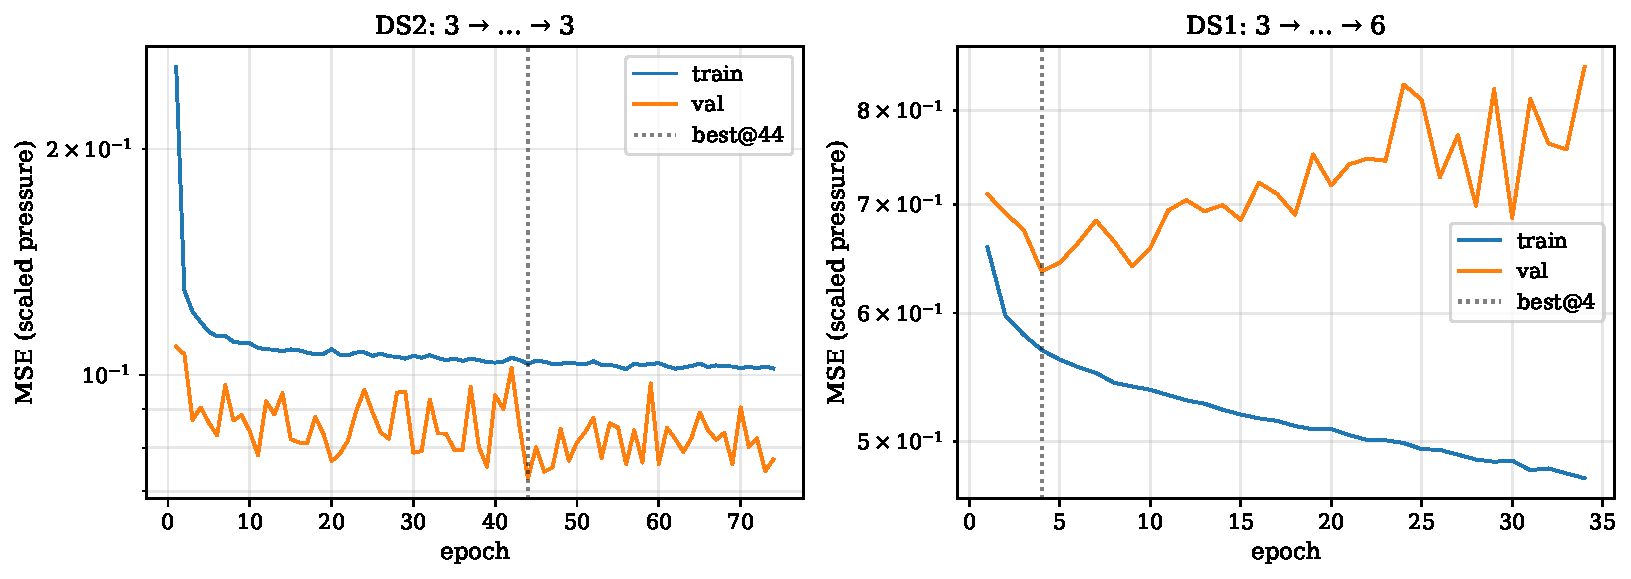
\includegraphics[width=0.92\linewidth]{fig/mlp_training_curves.pdf}
  \caption{Training and validation pressure MAE as a function of epoch for the tip-only MLP on Dataset~1 (left) and Dataset~2 (right). Vertical dashed lines mark the early-stopping best-epoch indices reported in Table~\ref{tab:app_hyperparams_networks}.}
  \label{fig:app_training_curves}
\end{figure}

Figure~\ref{fig:app_mlp_sweep} presents the hyperparameter sweep heatmap referenced in Section~\ref{sec:hparam_sweep}. Each cell reports the validation pressure MAE at the corresponding $(\text{hidden width}, \text{learning rate})$ combination on Dataset~2; the $128$-unit, $10^{-3}$ configuration chosen for all subsequent experiments is inside the region of flat near-optimal performance.

\begin{figure}[!htbp]
  \centering
  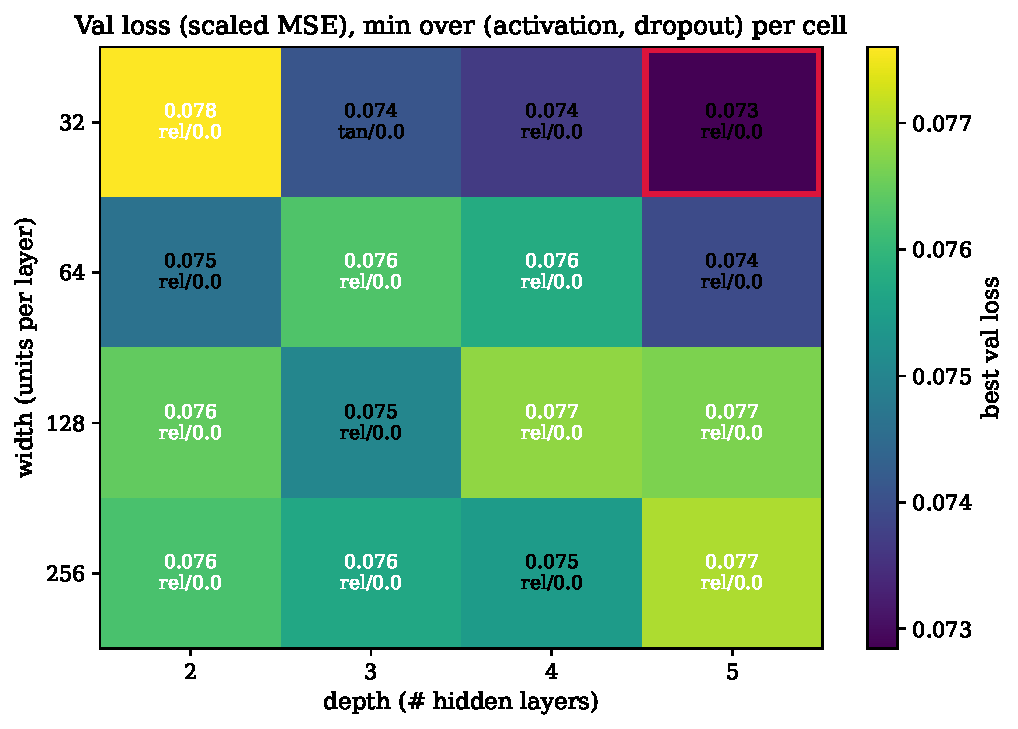
\includegraphics[width=0.78\linewidth]{fig/mlp_sweep_heatmap.pdf}
  \caption{Validation pressure MAE across the MLP hyperparameter sweep on Dataset~2. Darker cells denote lower error. The configuration selected for all reported MLP experiments is marked with a white frame.}
  \label{fig:app_mlp_sweep}
\end{figure}

Figure~\ref{fig:app_jacobian_time} shows the per-target inference-time distribution of the Jacobian-learned iteration on Dataset~1, as referenced in Section~\ref{sec:res_jacobian_efficiency}. The horizontal axis is logarithmic; the distribution is bimodal, with a left mode corresponding to targets that reach the $1$\,mm tolerance within the first few iterations (typical of warm-started trajectories) and a right mode corresponding to cold-start or near-singular targets that consume the full iteration cap.

\begin{figure}[!htbp]
  \centering
  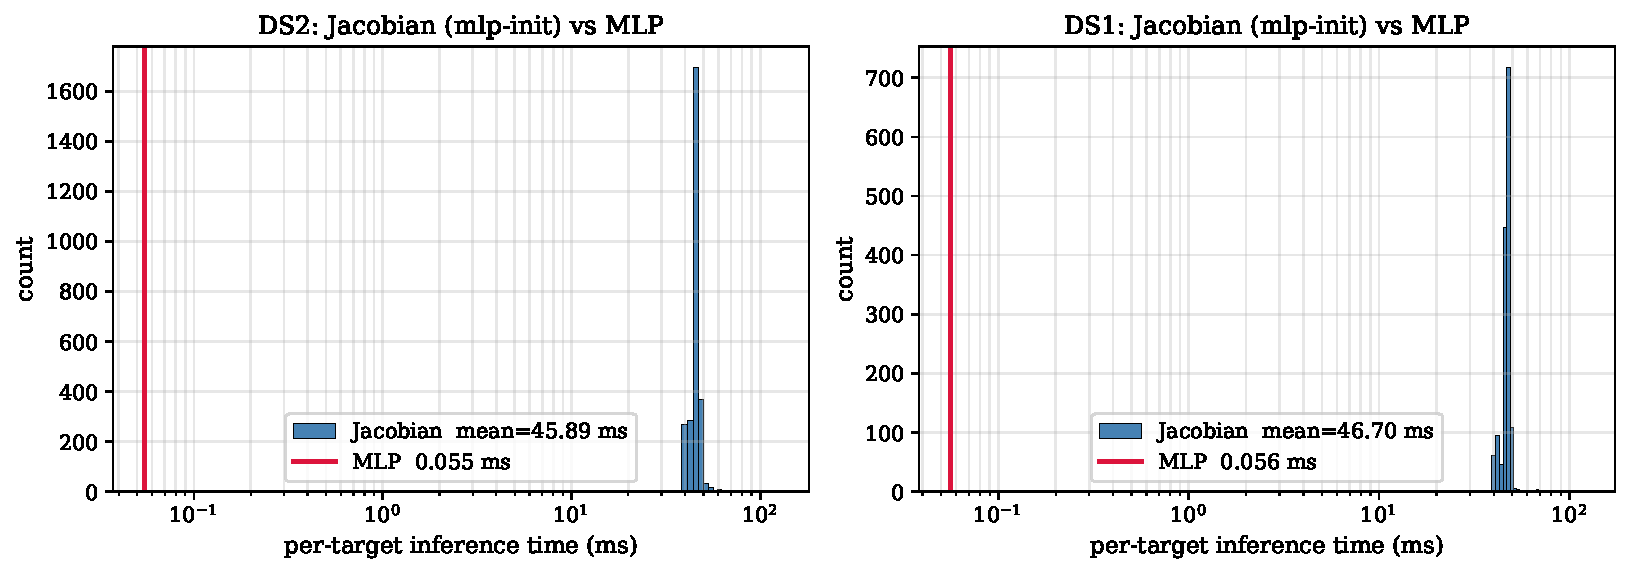
\includegraphics[width=0.78\linewidth]{fig/jacobian_inference_time.pdf}
  \caption{Distribution of per-target wall-clock inference time for the Jacobian-learned iteration on Dataset~1. Horizontal axis is logarithmic (milliseconds). The left mode corresponds to warm-started targets; the right mode to cold-start or near-singular targets that saturate the $50$-iteration cap.}
  \label{fig:app_jacobian_time}
\end{figure}

\section{Reproducibility}
\label{app:reproducibility}

Table~\ref{tab:app_repro_env} lists the software and hardware environment in which every experiment of Chapter~\ref{chap:results} was executed. All numbers reported in this thesis were generated on this single workstation with a fixed random seed of $42$ and cuDNN set to deterministic (\texttt{deterministic=True}, \texttt{benchmark=False}); re-running the training scripts in the same environment reproduces the tabulated metrics to within the last displayed digit.

\begin{table}[!htbp]
  \centering
  \small
  \caption{Software and hardware environment used for all experiments.}
  \label{tab:app_repro_env}
  \begin{tabularx}{\linewidth}{@{}l X@{}}
    \toprule
    Component & Value \\
    \midrule
    Operating system        & Ubuntu 24.04.4 LTS (Linux 6.17.0) \\
    CPU                     & Intel Core i7-13650HX (14 cores, 20 threads) \\
    RAM                     & 16\,GB DDR5 \\
    GPU                     & NVIDIA GeForce RTX 4060 Laptop (8\,GB, CUDA 12.6) \\
    Python                  & 3.11 \\
    PyTorch                 & 2.11.0+cu126 \\
    torchvision             & 0.26.0+cu126 \\
    NumPy / Pandas / SciPy  & 2.4.3 / 3.0.2 / 1.17.1 \\
    scikit-learn            & 1.8.0 \\
    matplotlib              & 3.10.8 \\
    PyElastica              & 0.3.3.post2 \\
    Random seed             & $42$ (Python, NumPy, PyTorch CPU and CUDA) \\
    cuDNN flags             & \texttt{deterministic=True}, \texttt{benchmark=False} \\
    Outer repository commit & \texttt{e9a7d5d} (\textit{soft\_robot\_ai}) \\
    \bottomrule
  \end{tabularx}
\end{table}

\paragraph{Checkpoint layout.}
All trained networks are stored under \texttt{checkpoints/\{experiment\}/\{run\_id\}/best.pt}, where \texttt{experiment} is one of \{\texttt{mlp\_ds1\_tip}, \texttt{mlp\_ds1\_tipmid}, \texttt{mlp\_ds2\_tip}, \texttt{lstm\_ds1\_tip}, \texttt{lstm\_ds1\_tipmid}, \texttt{lstm\_ds2\_tip}, \texttt{fk\_ds1}, \texttt{fk\_ds2}, \texttt{sim2real\_A}, \texttt{sim2real\_B}, \texttt{sim2real\_C}\} and \texttt{run\_id} encodes the date and the configuration hash. Each checkpoint file is a single PyTorch dictionary with keys \texttt{model\_state\_dict}, \texttt{optimizer\_state\_dict}, \texttt{config} (the full YAML used for training), \texttt{input\_scaler}, \texttt{output\_scaler}, \texttt{seed}, \texttt{git\_hash}, and \texttt{timestamp}, following the metadata convention of Section~\ref{sec:training_protocol}.

\paragraph{Evaluation determinism.}
Evaluation scripts load the checkpoint, restore both scalers, re-seed all random-number generators, and run a single forward pass over the frozen test split. No test-time augmentation, dropout, or batch-normalisation update is applied. Closed-loop tracking evaluations use the fixed reference trajectories of Section~\ref{sec:trajectory_tracking} and the same FK arbiter checkpoint for every method, so that any differences between methods are attributable to the methods themselves rather than to arbiter variation.

\paragraph{Code availability.}
The training scripts, evaluation pipelines, configuration files, and figure-regeneration scripts are archived in the project repository described in Appendix~\ref{app:code}. The exact commit associated with the numbers reported in Chapter~\ref{chap:results} is \texttt{e9a7d5d} on the \texttt{master} branch; the raw Dataset~1 pickles and the Dataset~2 CSV are held under \texttt{data/raw/} and are not redistributed because of upstream licensing constraints stated in Appendix~\ref{app:code}.
